\chapter{Detailed descriptions of the metadata normalization procedures }\label{app:1}

\section{Detailed description of ontology term mapping pipeline } \label{sec:mapping_pipeline}

\begin{enumerate}
\item \textbf{Initializing the Text Reasoning Graph (TRG):} The initial TRG consists of a set of nodes that represent the raw set of key-value pairs describing the sample.  First, a node is created for each key-value pair.  From each of these ``start nodes'', we draw two edges to two artifact nodes -- one artifact representing the key and the other artifact representing the value.  Figure~\ref{fig:init_trg} depicts the initial TRG for the following set of key value pairs:
\begin{align*}
    &\text{\texttt{cell line: Parkin-expressing MRC5 fibroblasts}}\\
    &\text{\texttt{cell state: Proliferating}}\\
    &\text{\texttt{source\_name: Prolif}}
\end{align*}

\begin{figure}[htbp]
\centering
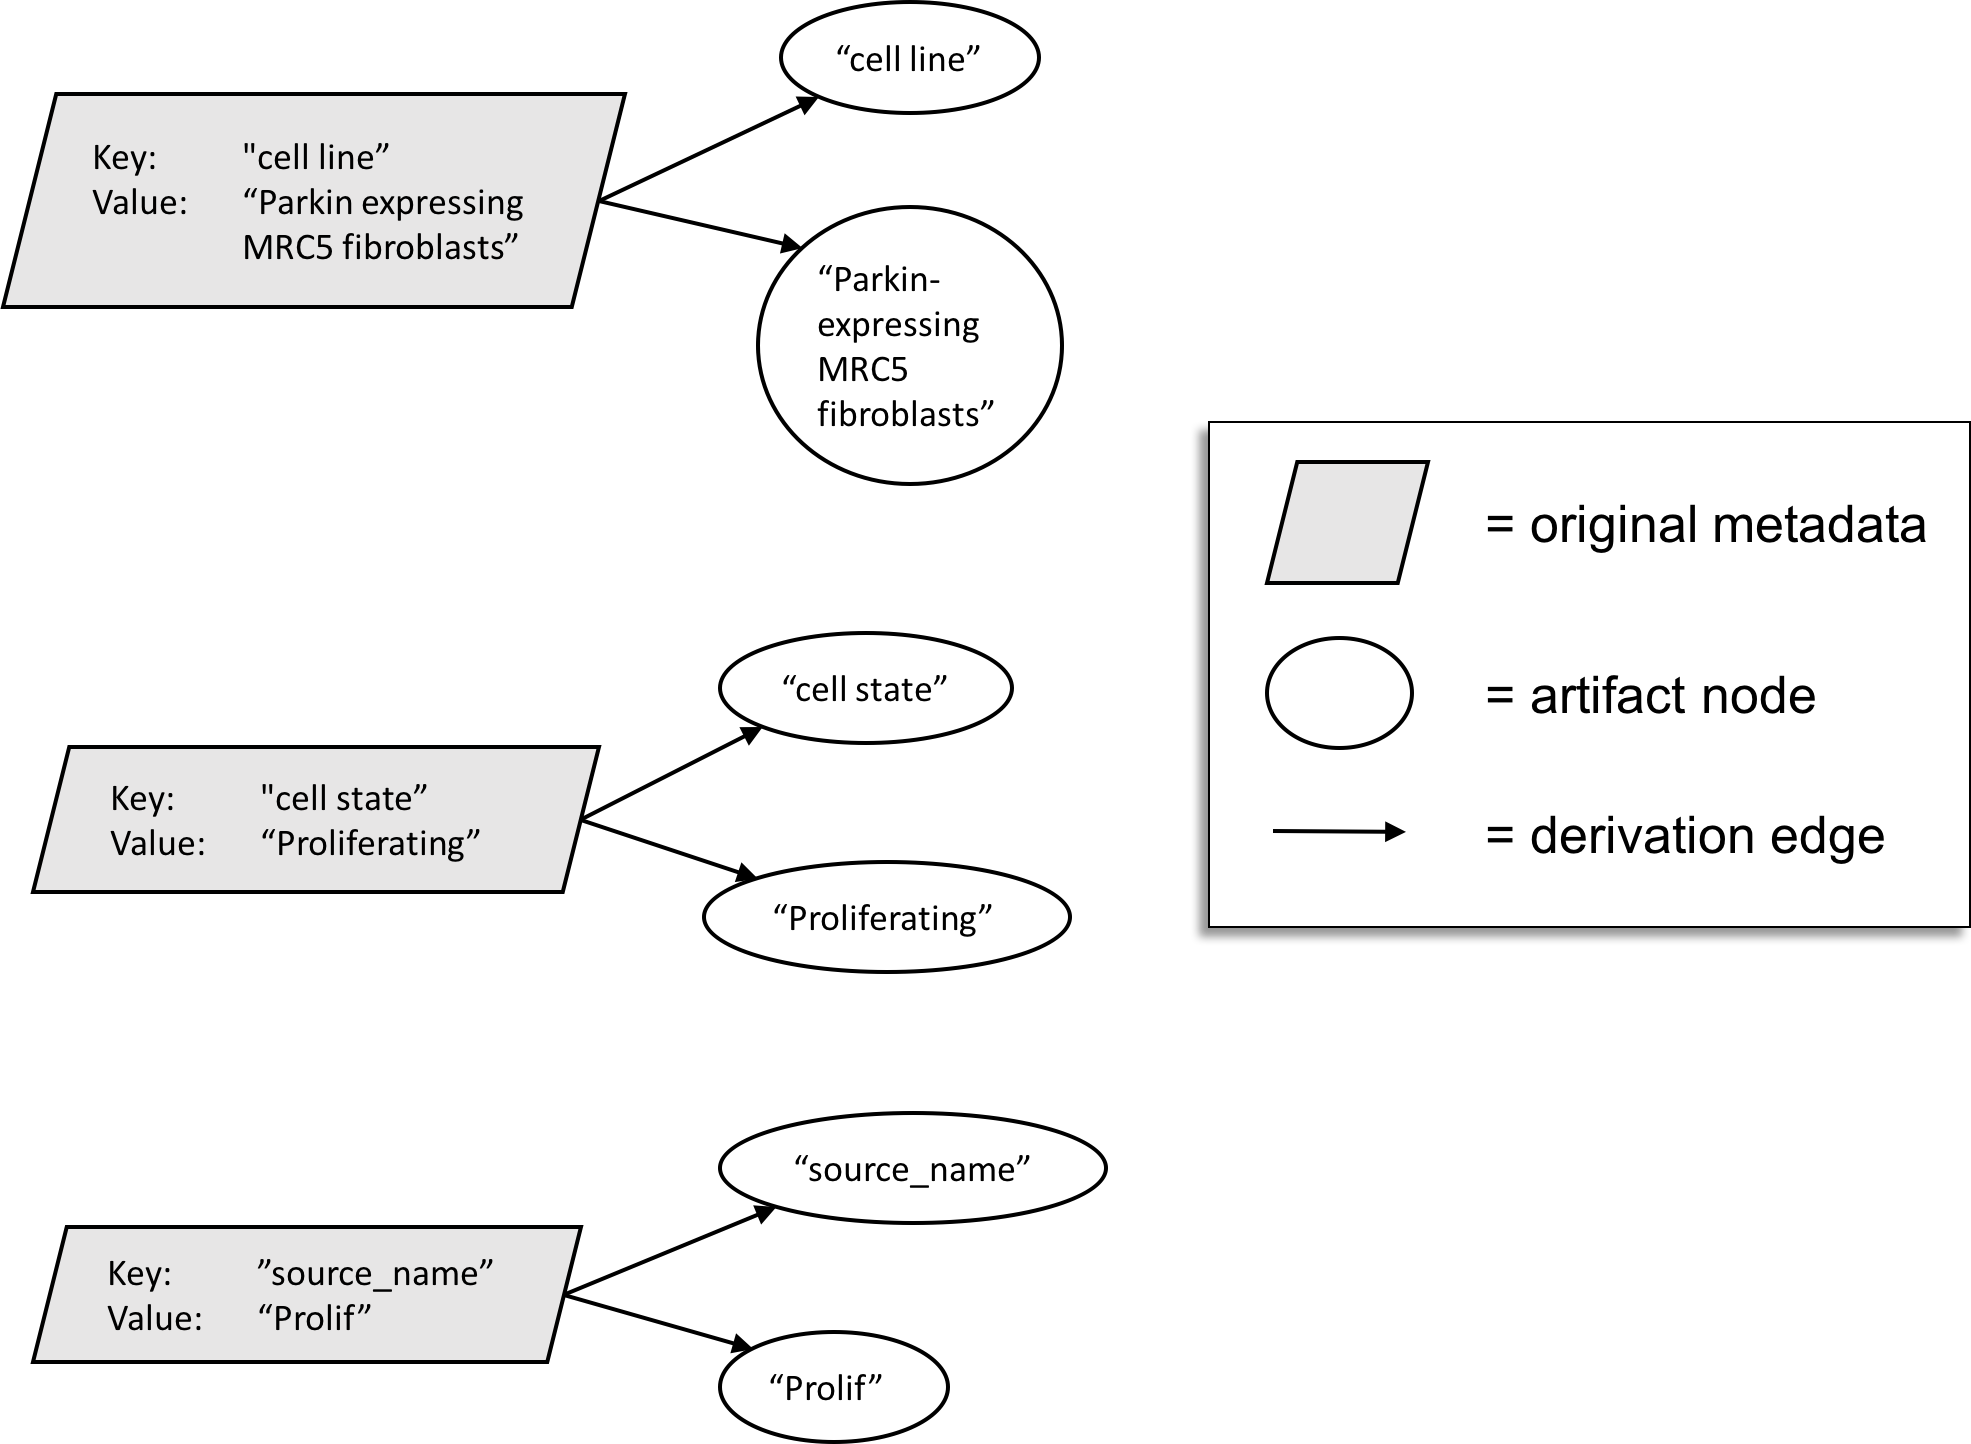
\includegraphics[width=13cm]{figures/init_trg.png}  
\caption{\textbf{Initial TRG.} The initial TRG created from a set of key-value pairs describing a sample.}
\label{fig:init_trg}
\end{figure}

\item \textbf{Generating $n$-grams:} From each artifact node, we generate all $n$-grams for $n = 1,\dots,8$. We use the Python Natural Language Toolkit (nltk) to tokenize the text before constructing $n$-grams.  For each $n$-gram generated from an artifact, we draw an edge from the original artifact to the derived artifact. Figure~\ref{fig:stages_1}A illustrates an artifact node from the graph of Figure~\ref{fig:init_trg} with derived artifacts representing $n$-grams. 

\begin{figure}[htbp]
\centering
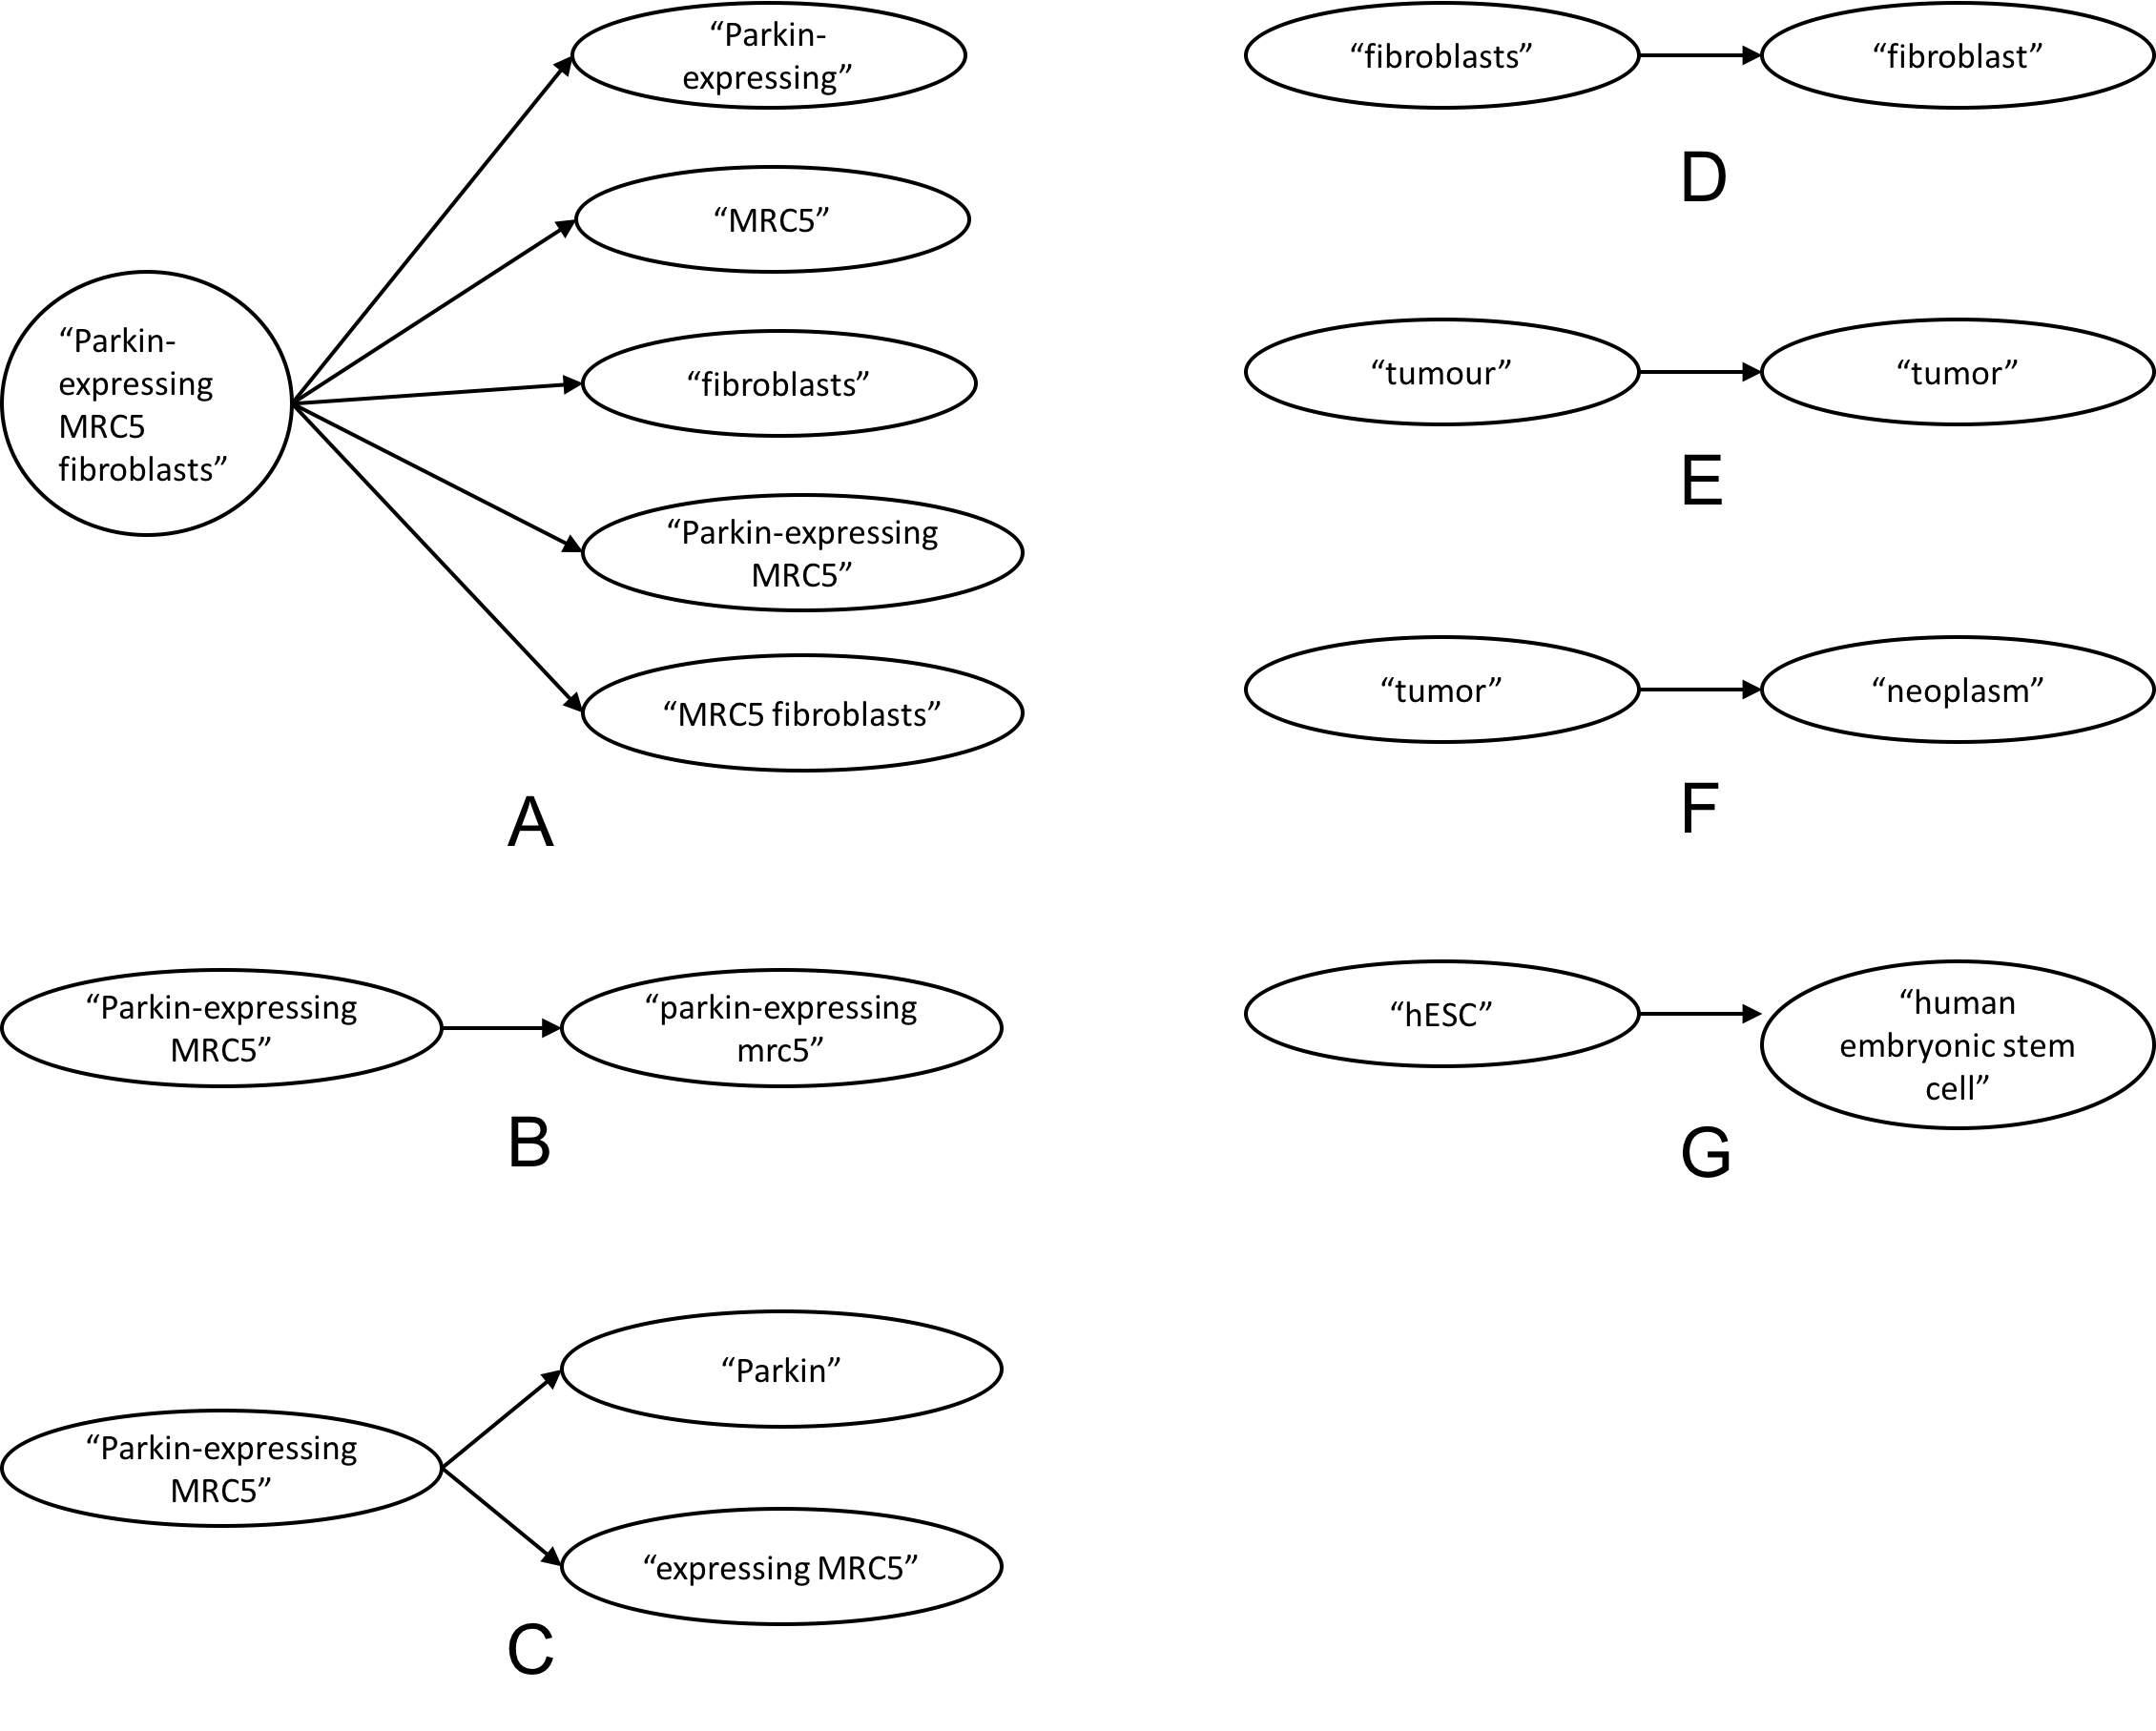
\includegraphics[width=13cm]{figures/stages_1.png} 
\caption{\textbf{Artifact derivations.} (A) An artifact node with derived $n$-grams. (B) An artifact with a derived lowercase artifact. (C) Delimiting artifacts on special characters. (D) Deriving inflectional variants. (E) Deriving spelling variants. (F) Deriving custom synonyms. (G) Expanding acronyms.}
\label{fig:stages_1}
\end{figure}

\item \textbf{Lowercase:} From each artifact node that represent artifacts with uppercase characters, we draw an edge to a new artifact node that has all lowercase characters. Figure~\ref{fig:stages_1}B demonstrates this process.

\item \textbf{Delimiters:} The NLTK's tokenizer does not split on the characters ``+'', ``-'', ``/'', and ``\_''.  We therefore, split all artifact strings by these delimiters as shown in Figure~\ref{fig:stages_1}C.  

\item \textbf{Inflectional variants:} We derive the inflectional variants of all artifacts by consulting the SPECIALIST Lexicon. This is demonstrated in Figure~\ref{fig:stages_1}D.

\item \textbf{Spelling variants:} We derive the spelling variants of all artifacts by consulting the SPECIALIST Lexicon. This is demonstrated in Figure~\ref{fig:stages_1}E.

\item \textbf{Manually annotated synonyms:} There are certain words that are very common in the metadata, but that are not included in the ontologies. For example, the word ``tumor'' is extremely common in the metadata, but is not present in the Disease Ontology. We filled such gaps by creating a small, custom thesaurus.  In our thesaurus, ``tumor'' is given the synonym ``neoplasm.'' The word ``neoplasm'' is a term in the Disease Ontology that is semantically equivalent to ``tumor.''  This process is demonstrated in Figure~\ref{fig:stages_1}F.

\item \textbf{Custom acronym expansion:} There are certain acronyms that are common in the metadata, but are not included in the ontologies. For example, the acronym ``hESC'' is very common in the metadata, but is not present in the Cell Ontology.  We filled such gaps by expanding common acronyms. For example, we expand ``hESC'' to ``human embryonic stem cell.'' This process is demonstrated in Figure~\ref{fig:stages_1}G.  

\item \textbf{Exact string matching:} We perform a preliminary mapping step in which we map artifacts to ontology terms by searching for exact matches between the artifact strings and term names and synonyms in the ontologies. This preliminary mapping stage is performed quickly using a trie data structure.

\item \textbf{Context-specific synonyms:}  We create a list of ``context-specific synonyms'' and derive synonyms for artifacts when that artifact was derived from a value that is associated with a specific key. For example, a common key-value pair is \texttt{sex: F}.  Here, the string ``F'' is an abbreviation for ``female''; however, this is only known because the key maps to the EFO term for ``sex.'' ``F'' in another context may not be an abbreviation for ``female.'' This process is illustrated in Figure~\ref{fig:context_syn}.  

\begin{figure}[htbp]
\centering
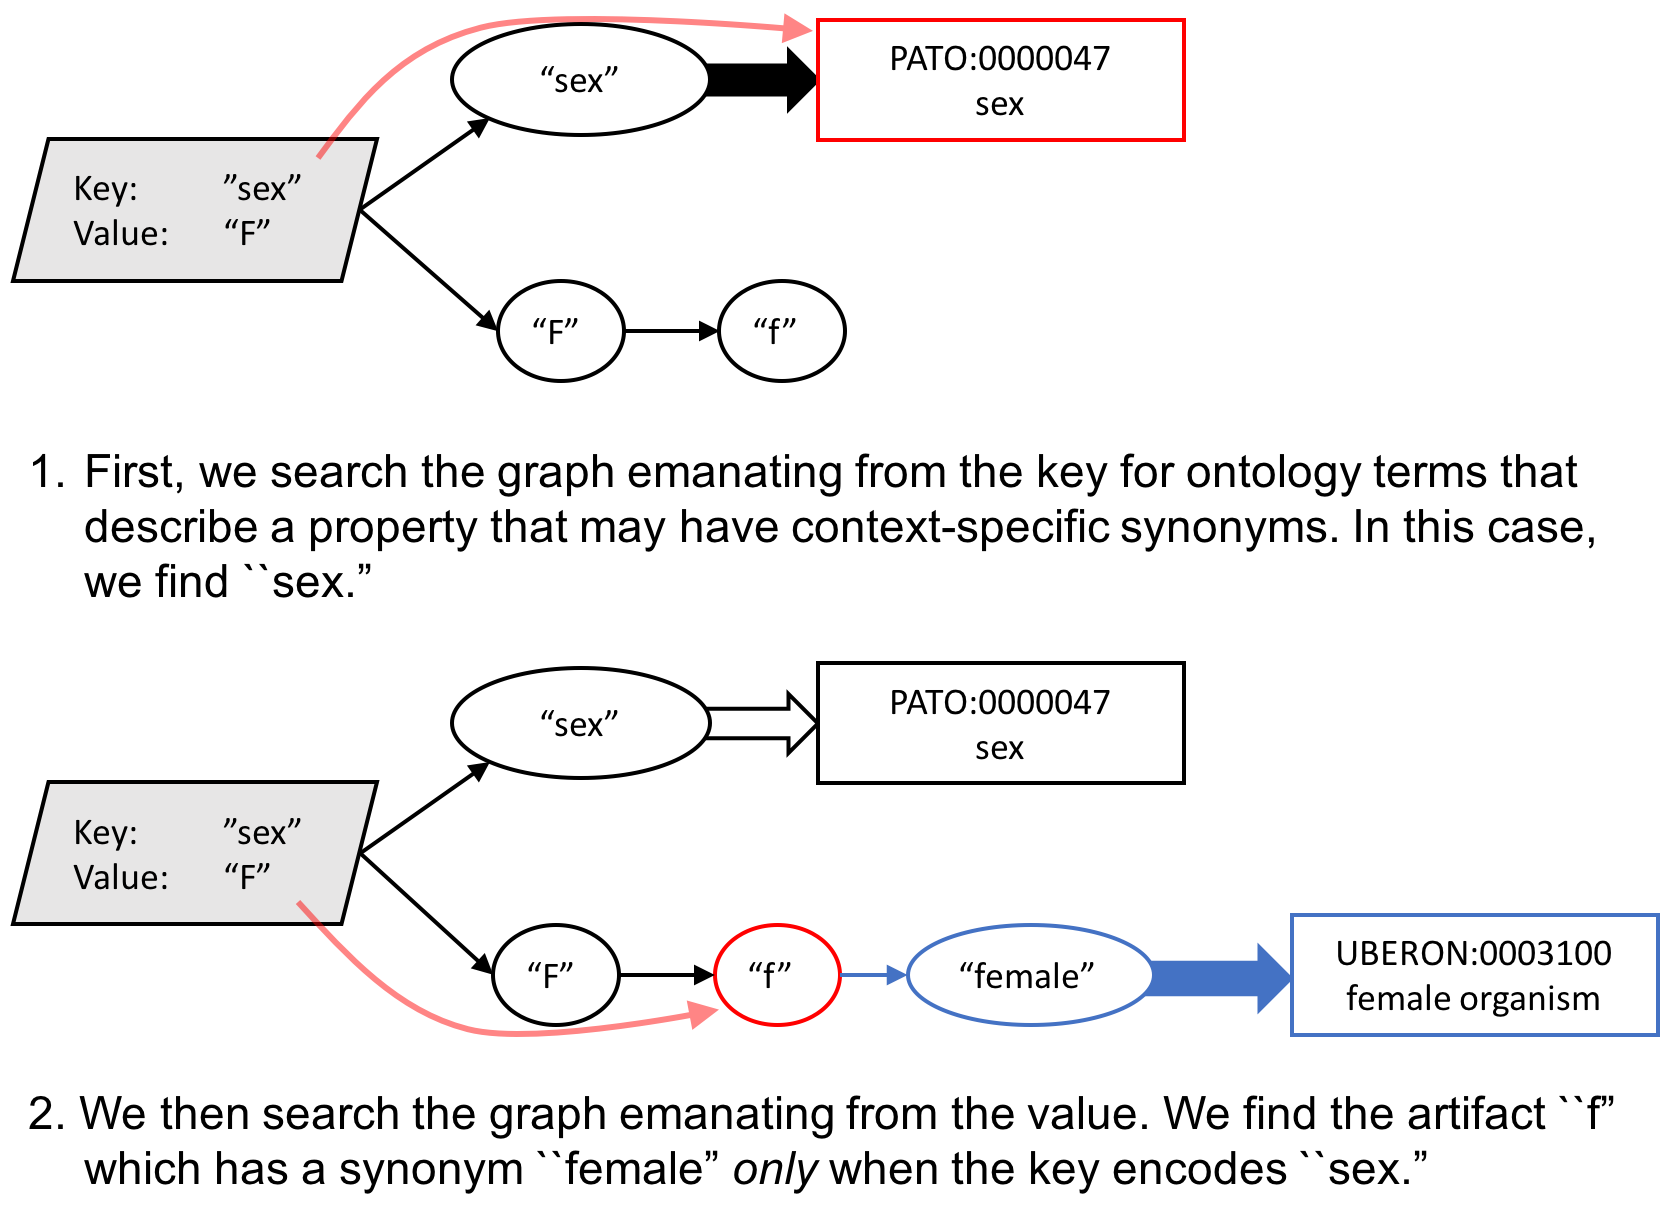
\includegraphics[width=11cm]{figures/context_specific_synonyms.png} 
\caption{\textbf{Extracting context-specific synonyms.} An example describing context specific synonyms.}
\label{fig:context_syn}
\end{figure}

\item \textbf{Fuzzy string matching} We perform fuzzy string matching between the artifacts and the ontology terms.  Let $a$ and $b$ be two strings and let $d(a, b)$ be their Levenshtein edit distance. Let $l(x)$ be the length of a string $x$. An artifact $a$ matches with an ontology term name or synonym $b$ if the following conditions hold: $l(a) > 2$, $d(a,b) \leq 2$, and $d(a,b) \leq \text{max}\{l(a), l(b)\} / 10$. We do not match artifacts that are less than 3 characters long in order to avoid false positive mappings.  If the artifact is greater than 2 characters long, a match is called if the edit distance is less than or equal to 2 and less than or equal to 0.1 times the length of the longer string. For example, the misspelled artifact ``forskin fibroblast'' would match with the ontology term name ``foreskin fibroblast.''  In contrast, the string ``year'' would not match with the ontology term ``ear'' because the edit distance of 1 is greater than 0.1 of the length of the longer string.  When an artifact matches an ontology term, we create a node representing the ontology term and draw an edge from the artifact to the new ontology term node. 

To more efficiently perform fuzzy string matching we store all ontology term names and synonyms in a Burkhard-Keller metric tree \cite{Burkhard} with the bag-distance metric defined in \cite{Bartolini}.  When performing fuzzy string matching between a query string $s$ and the strings in the metric tree, we retrieve all strings in the metric tree that are within a distance of 2 from $s$ using bag-distance. Since bag-distance is a lower-bound on edit-distance, this process filters out all strings in the ontologies whose lower bound on the edit distance is greater than the threshold of 2 that we impose on fuzzy string matching.  We then explicitly compute edit distance between $s$ and the retrieved strings. 

\item \textbf{Matching to custom terms:} There are several noun-phrases that are common in the metadata and that are superstrings of ontology terms, but that do not imply that the sample maps to the contained ontology term.   For example, the phrase ``blood type'' does not imply that the sample was derived from blood.  Similarly, ``tissue bank'' describes the organization that provided the sample, but does not necessarily imply that the sample is a tissue sample. To differentiate the larger noun-phrase from the ontology term it contains, we maintain a custom list of misleading noun-phrases and remove ontology term mappings if those mappings were derived from a substring of a misleading noun-phrase. For example, given the string ``blood type'', the artifact ``blood'' will be blocked from mapping to the ontology term for blood because it is a substring of the noun-phrase ``blood type.'' Currently, we have 27 noun-phrases in our index and we will continue to build this index as we find more misleading noun-phrases that contain ontology terms.


\item \textbf{Remove extraneous cell-line matches:} 
Many cell lines have short names that oftentimes resemble acronyms or gene names.  For example, ``SRF'' is a gene as well as a cell line in the Cellosaurus. Similarly, ``MDS'' is often used as an acronym for Myelodysplastic Syndromes and also happens to be the name of a cell line in the Cellosaurus.

We remove extraneous mappings to cell line terms by searching the graph emanating from the key for a lexical match to ontology terms such as those for ``cell line'' and ``cell type''.  If such a match is \textit{not} found, we search the graph emanating from the value for artifacts that have a lexical match to a cell line ontology term and remove all such ontology term nodes.  This process is illustrated in Figure~\ref{fig:block_cell_line}.

\begin{figure}[htbp]
\centering
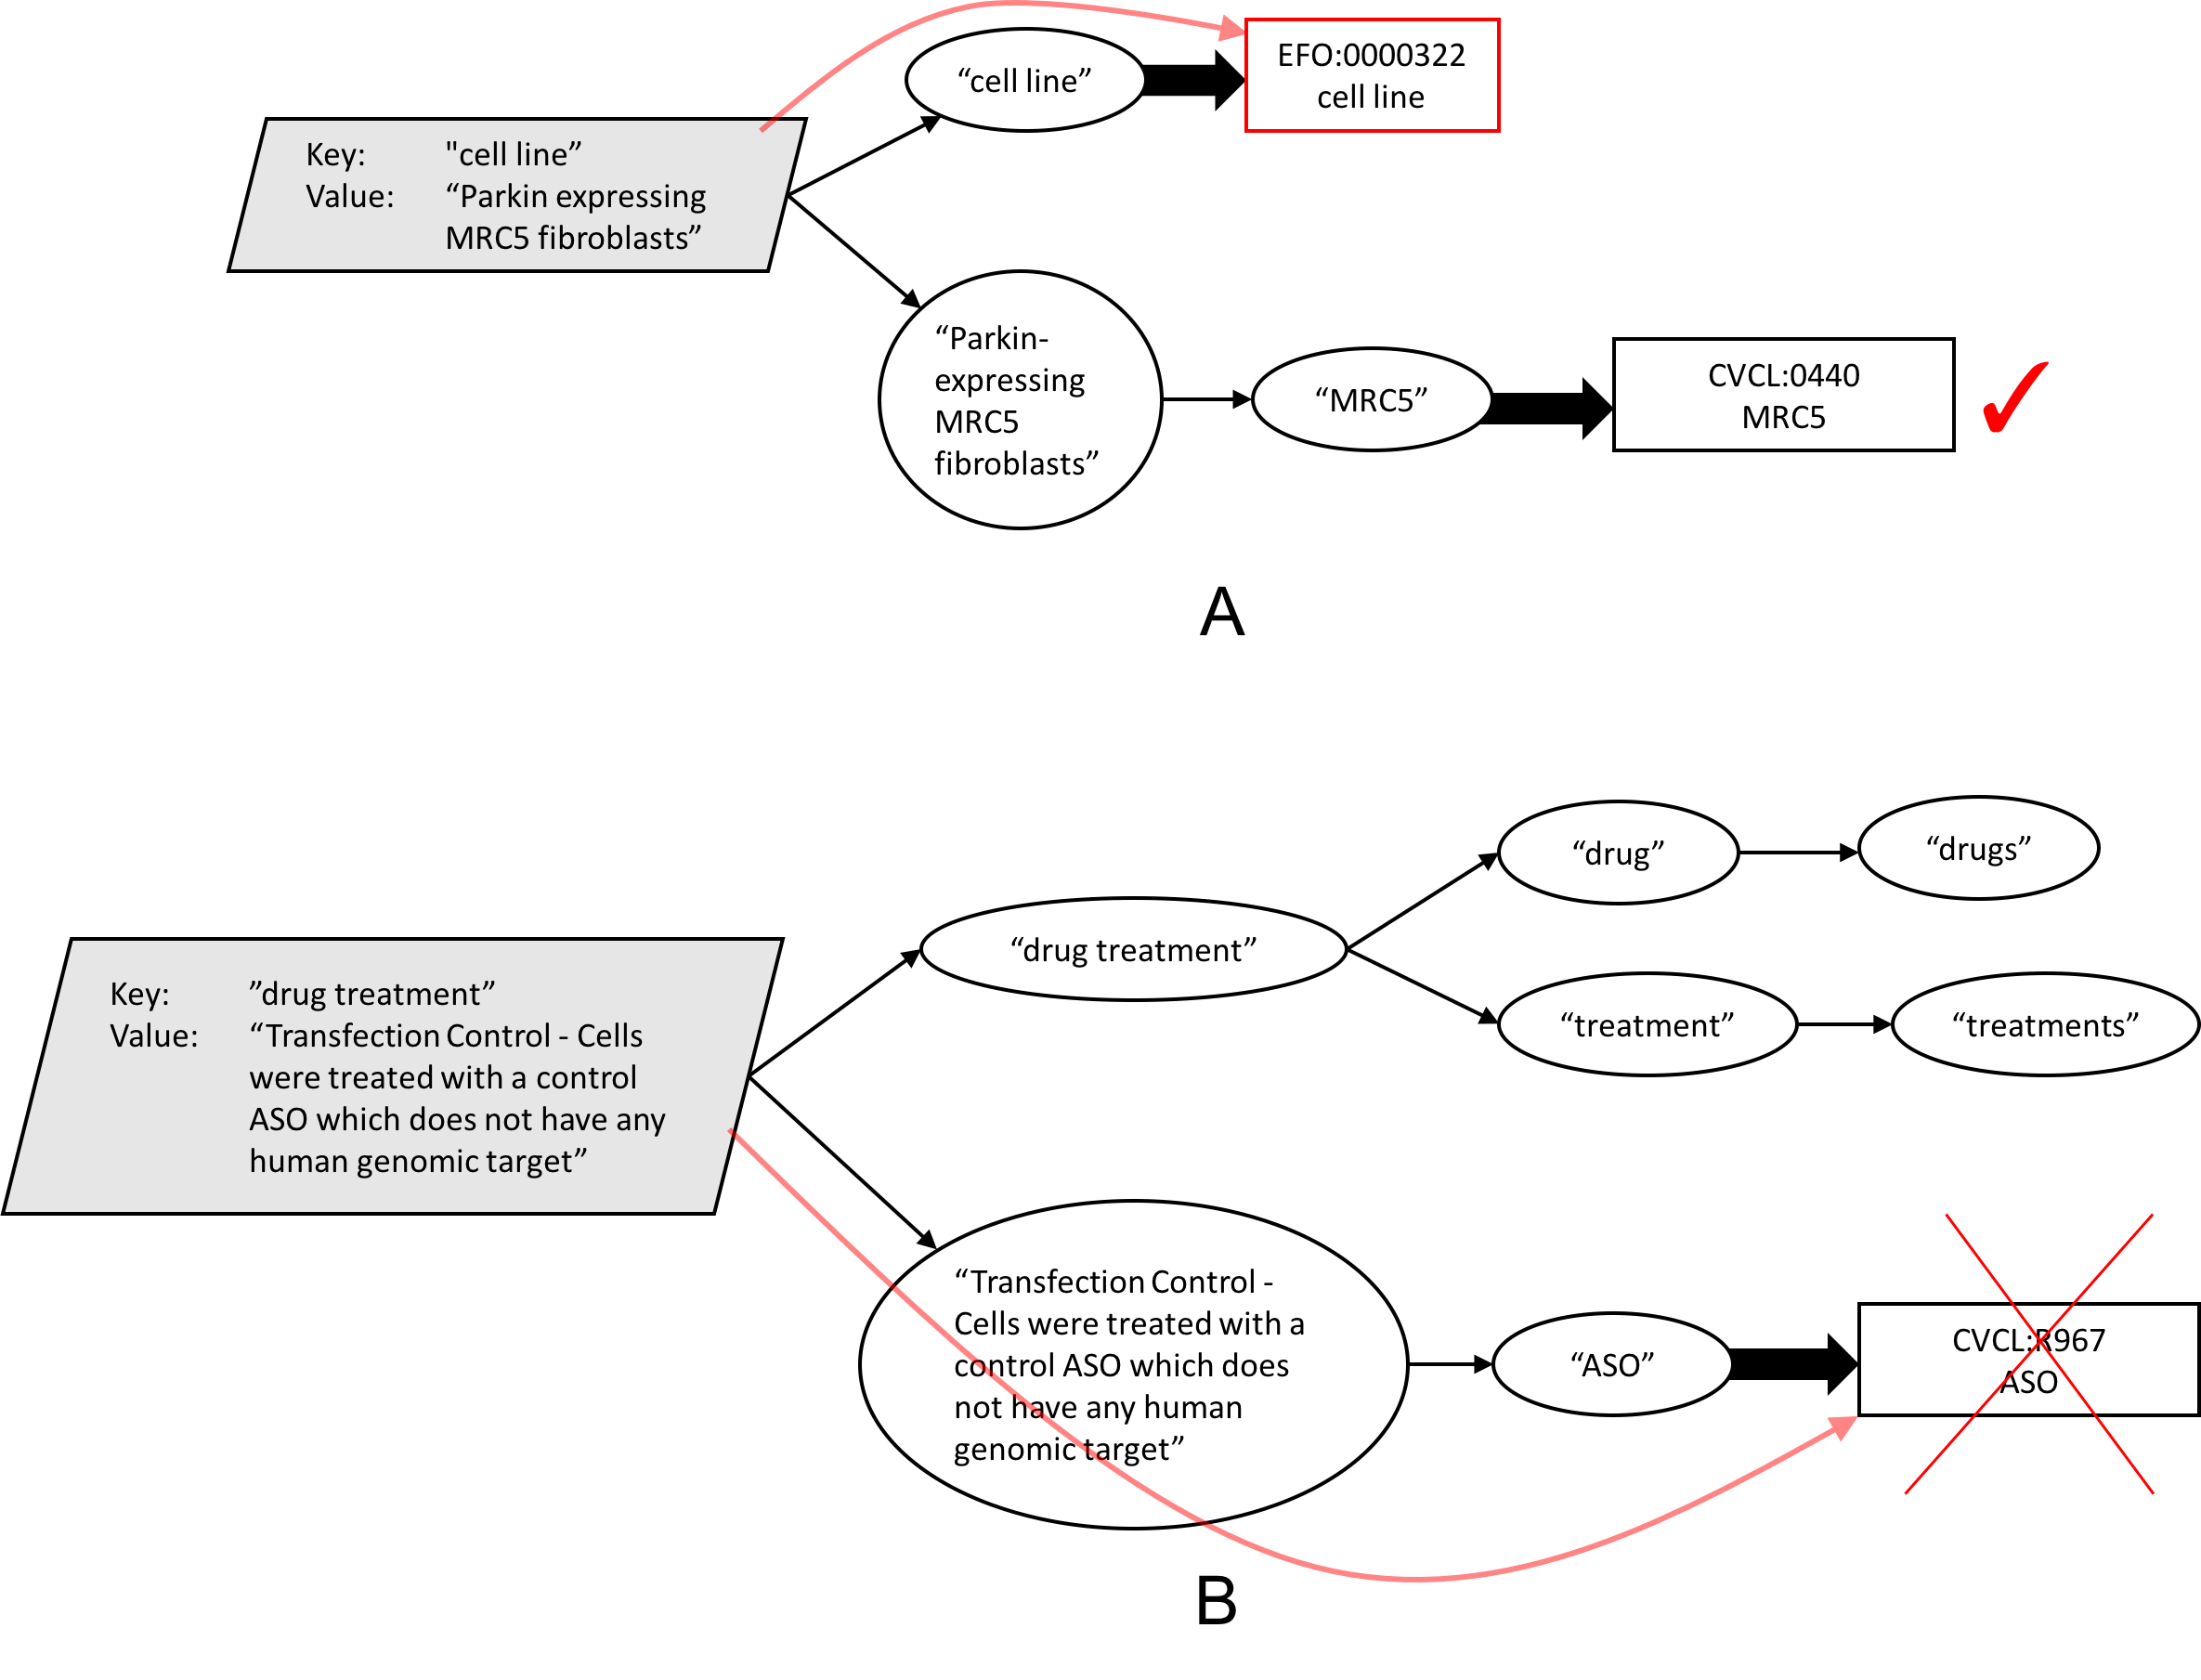
\includegraphics[width=13cm]{figures/block_cell_line.png} 
\caption{\textbf{Removing extraneous cell line terms.} (A) The term ``cell line'' was found in the graph emanating from the key.  Thus, we keep the cell line term for ``MRC5'' in the graph emanating from the value. (B) No ontology term for ``cell line'' or ``cell type'' was found in the graph emanating from the key. We therefore remove the cell line term for ``ASO'' in the graph emanating from the value.}
\label{fig:block_cell_line}
\end{figure}


\item \textbf{Map to linked-superterms:} The domain covered by the EFO overlaps with many of the other ontologies because it includes cell types, anatomical entities, diseases, and cell lines.  In many cases, the EFO is inconsistent with other ontologies in how it draws edges between terms.  For example, the term ``lung adenocarcinoma'' and ``adenocarcinoma'' are present in both the Disease Ontology and the EFO; however ``adenocarcinoma'' is a parent of ``lung adenocarcinoma'' only in the Disease Ontology and not in the EFO.  These inconsistencies pose a problem when we filter for the maximal phrase-length in the metadata.   For example, when a sample maps to ``lung adenocarcinoma'' and ``adenocarcinoma'', we remove ``adenocarcinoma'' because it is a substring of ``lung adenocarcinoma''.  This is valid for the Disease Ontology because the term for ``adenocarcinoma'' is implied by ``lung adenocarcinoma'' by its position in the ontology.  However, this results in a false negative for the EFO version of this term.  

To counteract this problem, we link the terms in the EFO to terms in the other ontologies.  Two terms are linked when they share the same term-name or exact-synonym.  Then, when an artifact maps to a term, we traverse the term's ancestors and map to any terms that are linked to those ancestors.   In the case of ``lung adenocarcinoma'', we would traverse the ancestors of this term in the Disease Ontology and map to the EFO's ``adenocarcinoma'' because it is linked to the Disease Ontology version of this term. Figure~\ref{fig:linked} illustrates this process. 


\item \textbf{Cell line disease implications:} The EFO is missing edges between disease cell line terms and the corresponding disease terms. For example, the term ``cancer cell line'' does not have an edge to ``cancer.''  To fill this gap, if a sample maps to a cell line category term, we also map to the corresponding disease terms. 


\item \textbf{Block superterm mapping:} It is a common occurrence for disease ontology terms to include anatomical entities in their name. For example, ``breast cancer'' includes ``breast'' as a substring. It would be incorrect to map ``breast'' to the sample because this word localizes the cancer, but does not localize the origin of the sample.  We note that it is possible that the sample was indeed derived from breast tissue; however, it is also possible the sample originated from other tissue such as a malignant site.  We maintain a conservative approach and avoid mapping to ``breast.''  We implement this process by designing each artifact node to keep track of the original character indices in the metadata from which it was derived. After mapping all artifacts to the ontologies, we remove all ontology terms that were lexically matched with an artifact node that is subsumed by another artifact node that matches with another ontology term.  

\item \textbf{Custom consequent mappings:}  We maintain a small list of 6 common terms that imply other terms.  For example, if a cell maps to a the EFO term for ``cell line'', we consequently map the sample to the Cell Ontology's term for ``cultured cell.''  

\item \textbf{Real-value property extraction:} We maintain a list of ontology terms that define real-value properties. Currently, we use 6 terms: ``age'', ``passage number'', ``timepoint'', ``age at diagnosis", ``body mass index", and ``age at death."  Future work will entail expanding this list.  To extract a real-value property from a key-value pair, we search the graph emanating from the key for a match to a property ontology term.  If such a property is found, we search the graph emanating from the value for an artifact representing a numerical value and a unit ontology term node (e.g., ``46'' and ``year'').  From this process, we extract the triple (property, value, unit). For example, given the key-value pair \texttt{age: 46 years old}, we extract (``age'', 46, ``year'').


\item \textbf{Filtering mapped ontology terms by semantic similarity:}
The ontologies are structured so that each synonym of an ontology term is given a synonym-type. These types include ``exact'', ``broad'', and ``narrow.'' These synonym-types describe the relationship between the synonym string and the term name.  An ``exact'' synonym indicates that the string is semantically closer to the ontology term name than a ``broad'' synonym.  If an artifact matches to multiple ontology terms, the ontology term with the semantically nearest matched target is likely to be the best match with the artifact. Thus, given an artifact with multiple matched terms, we examine the targets within the matched terms to which the artifact matched and rank these targets according to the semantic similarity with the ontology term name.  We then keep the match with the highest similarity and discard the rest.  

For example, given the artifact ``skin'', we find several terms in the Uberon ontology that have a synonym ``skin'':  ``zone of skin'' (exact synonym), ``skin epidermis'' (broad synonym), ``skin of body'' (related synonym), and ``integument'' (related synonym). Of these terms, ``skin'' is semantically most similar to the term ``zone of skin'' because it is an exact synonym of this term.  We therefore keep this mapping and discard the rest.

\item \textbf{Consequent cell line mappings:} Our pipeline draws edges between cell line ontology term nodes and the ontology terms that describe the cell line.   For example, if the TRG contains the node for the cell line ``HeLa'', we draw an edge to the ontology terms for ``adenocarcinoma'' and ``female'' because this cell line was derived from a woman with cervical adenocarcinoma.  We consider such mappings to be consequent mappings because they are retrieved using an external knowledge base.   
 
 This knowledge base was created from data we scraped from the ATCC website at \url{https://www.atcc.org}. To construct mappings between cell lines and ontology terms, we ran a variant of our pipeline on the scraped cell line data.  We scraped cell line metadata for all cell lines that are present in the Cellosaurus. 

\item \textbf{Consequent developmental stage mappings:} If the sample maps to a real-value property with property ``age'' and unit ``year'', we check whether the value is greater than 18. If so, we consequently map the sample to the EFO and Uberon terms for ``adult.''
\end{enumerate}


\section{Detailed description of sample-type prediction procedure } \label{sec:sample_pred}

Although we train a one-vs-rest classifier using logistic regression binary classifiers, we ultimately use a custom decision procedure for making a sample-type prediction.  This procedure entails limiting the possible predicted sample-types based on ontology terms that were mapped by our computational pipeline.  The algorithm chooses among the remaining possible sample-types by selecting the sample-type with highest confidence according to the one-vs-rest classifier.    

To provide an example, if the ontology term ``stem cell'' was mapped to the sample, we set $p(y = j | x) = 0$ for $j \in \{\text{\texttt{ tissue, cell line, primary cells}}\}$.  We then compute the probabilities $p_i := \frac{p(y=i \mid x)}{\sum_h p(y = h \mid x)}$ for each $i$.  Our final prediction is then $\hat{y} = \text{argmax}_i p_i$. In summary, this process asserts that if ``stem cell'' mapped to the sample, then the sample must be either a stem cell sample, in vitro differentiated cell sample, or induced pluripotent stem cell sample. We let the classifier decide which is the most likely label among these possible labels. 

More specifically, we follow the following steps for making a prediction:
\begin{enumerate}
\item If the sample maps to ``xenograft'' (EFO:0003942), then we predict \texttt{ tissue} with confidence 1.0.
\item If the sample was passaged (i.e. maps to a real-value property tuple with property ``passage number'' and unit ``count''), then we assert the sample cannot be \texttt{ tissue}. If the number of passages is greater than 0, then we assert the sample cannot be \texttt{ primary cell}.
\item If the sample maps to a cell line, then we check the Cellosaurus for the cell line category.  We map the Cellosaurus cell-line category to a set of possible sample types as follows:
\begin{itemize}
    \item Induced\_pluripotent\_stem\_cell: \texttt{ in vitro differentiated cells}, \texttt{ induced pluripotent stem cell line}
    \item Cancer\_cell\_line: \texttt{ cell line}
    \item Transformed\_cell\_line: \texttt{ cell line}
    \item Finite\_cell\_line: \texttt{ cell line}
    \item Spontaneously\_cell\_line: \texttt{ cell line}
    \item Embryonic\_stem\_cell: \texttt{ stem cells}, \texttt{ in vitro differentiated cells}
    \item Telomerase\_cell\_line: \texttt{ cell line}
    \item Conditionally\_cell\_line: \texttt{ cell line}
    \item Hybridoma: \texttt{ cell line}
\end{itemize}
\item If the sample maps to the term ``stem cell'', then we remove the possibility that the sample type is \texttt{ cell line}, \texttt{ tissue}, or \texttt{ primary cells}.  
\item If the sample maps to a specific cell-type term (i.e. any term that is a child of ``somatic cell''), then we remove the possibility that the sample-type is \texttt{ tissue}. This follows from our observation that when the metadata describes a specific cell-type, the sample consists of homogenous cells that have been isolated and filtered.  The sample no longer consists of cells positioned in their original three dimensional structure and is thus not a tissue sample.
\end{enumerate}






